\documentclass[12pt,a4paper]{article}
\usepackage[UTF8]{ctex}
\usepackage{amsmath,amssymb}
\usepackage{xcolor}
\usepackage{hyperref}
\usepackage{geometry}
\usepackage{graphicx}
\geometry{margin=2.5cm}

\title{Hidden Subgroup Problem / 隐子群问题}
\author{QuoNic}
\date{}

\begin{document}
\maketitle

\begin{center}
\textbf{Algorithms / 算法} | 难度：高级 | 预计时间：25 分钟
\end{center}

\tableofcontents
\newpage

\section{为什么需要？}

隐子群问题是量子计算的统一框架，许多量子算法都是它的特例。

\subsection{经典局限}
\begin{itemize}
  \item 经典算法需要指数时间求解隐子群问题
  \item 对于大群，经典方法效率低
\end{itemize}

\subsection{量子优势}
\begin{itemize}
  \item 量子算法可以在多项式时间内求解阿贝尔隐子群问题
  \item 提供指数加速
  \item 是许多量子算法的统一框架
\end{itemize}

\subsection{实际应用}
\begin{itemize}
  \item 大数分解（Shor 算法）
  \item 离散对数（Shor 算法）
  \item 图同构（量子算法）
\end{itemize}

\section{快速上手}

\begin{verbatim}
from quonic.algorithms import hsp

# 隐子群问题
result = hsp(group='Z4', oracle='period_finding')
print(f'Hidden subgroup: {result.subgroup}')
\end{verbatim}

\textbf{预期输出}：
\begin{verbatim}
Hidden subgroup: {0, 2}
\end{verbatim}

\section{原理详解}

\subsection{电路图}

\begin{center}
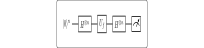
\includegraphics[width=0.6\textwidth]{../../images/hsp_circuit.svg}
\end{center}

\subsection{数学推导}

隐子群问题：
\begin{equation}
f: G \to X, \quad f(g) = f(h) \iff gH = hH
\end{equation}

其中 $H$ 是 $G$ 的子群，$f$ 是周期函数。

\textbf{量子算法}：
\begin{enumerate}
  \item 制备均匀叠加态
  \item 查询函数 $f$
  \item 用 QFT 提取子群信息
  \item 测量得到子群
\end{enumerate}

\subsection{几何解释}

隐子群问题在群空间中寻找隐藏的子群。量子叠加允许同时探索所有群元素。

\section{代码详解}

\begin{verbatim}
from quonic.algorithms import hsp

# hsp(group, oracle, n_qubits)
# group: 群类型
# oracle: 隐函数
# n_qubits: 量子比特数

result = hsp(
    group='Z4',
    oracle='period_finding',
    n_qubits=4
)

# result.subgroup: 隐子群
# result.generators: 生成元
# result.circuit: 量子电路
print(f'Hidden subgroup: {result.subgroup}')
\end{verbatim}

\section{进阶用法}

\subsection{场景 1：不同群}

\begin{verbatim}
from quonic.algorithms import hsp

# 不同群
result_z4 = hsp(group='Z4', oracle='period_finding')
result_z6 = hsp(group='Z6', oracle='period_finding')
result_d4 = hsp(group='D4', oracle='hidden_subgroup')

print(f'Z4 subgroup: {result_z4.subgroup}')
print(f'Z6 subgroup: {result_z6.subgroup}')
print(f'D4 subgroup: {result_d4.subgroup}')
\end{verbatim}

\subsection{场景 2：Shor 算法}

\begin{verbatim}
from quonic.algorithms import hsp

# Shor 算法是 HSP 的特例
result = hsp(group='Z_N', oracle='modular_exponentiation')
print(f'Period: {result.period}')
print(f'Factors: {result.factors}')
\end{verbatim}

\subsection{场景 3：图同构}

\begin{verbatim}
from quonic.algorithms import hsp

# 图同构问题
result = hsp(group='S_n', oracle='graph_isomorphism')
print(f'Isomorphic: {result.is_isomorphic}')
\end{verbatim}

\section{适用场景}

\subsection{大数分解}

隐子群问题是 Shor 算法的基础。Shor 算法用于大数分解，威胁 RSA 加密。

\subsection{离散对数}

隐子群问题是离散对数算法的基础。离散对数是许多密码系统的基础。

\subsection{图同构}

隐子群问题可以用于图同构问题。图同构是判断两个图是否结构相同的问题。

\section{常见问题}

\subsection{隐子群问题和 Shor 算法有什么关系？}

Shor 算法是隐子群问题的特例。Shor 算法求解的是整数分解问题，可以表示为隐子群问题。

\subsection{隐子群问题的难度如何？}

阿贝尔隐子群问题可以在多项式时间内求解，非阿贝尔隐子群问题仍然是开放问题。

\section{学习路径}

\subsection{前置知识}
\begin{itemize}
  \item 群论
  \item 量子傅里叶变换
  \item 量子相位估计
\end{itemize}

\subsection{继续学习}
\begin{itemize}
  \item Shor 算法
  \item 离散对数
  \item 后量子密码学
\end{itemize}

\section{完整示例代码}

\subsection{示例 1：基本隐子群问题}

\begin{verbatim}
from quonic.algorithms import hsp

result = hsp(group='Z4', oracle='period_finding')
print(f'Hidden subgroup: {result.subgroup}')
\end{verbatim}

\section{下载}

\begin{itemize}
  \item [hsp.py](https://github.com/ChrisLee0721/QuoNic/blob/main/examples/hsp/hsp.py)
\end{itemize}

\end{document}
